\subsection{Bandwidth Selection}

The previous section describes how we use the kernel density estimation method to calculate local crowd factors. The section mentions that the choice of bandwidth is crucial to the calculation.

%As kernel density estimation is not a new technique, much research has gone into bandwidth selection. This has resulted in many sophisticated approaches. \kanote*{forklar hvorfor vi ikke har det her focus, eller også vent med at fraskrive det, indtil det bliver forklaret i teksten}{We will in this project not focus on finding an optimal bandwidth using the best techniques known to research. Instead, we will do a simple bandwidth selection experiment that illustrates how different bandwidths affect the results of the kernel density estimation utilised in this project.}

We will in this section do a simple bandwidth selection experiment that illustrates how different bandwidths affect the results of the kernel density estimation utilised in this project.

\subsubsection{Undersmoothing and Oversmoothing}

The bandwidth is important because it controls how many data samples to include. There are two extremes: a too low bandwidth or a too high bandwidth. A too low bandwidth will cause the density estimation to be noisy; the estimate will have a big variance in its output. We call this an undersmoothed estimate. On the other extreme the bandwidth can be too high, meaning that too many data samples would be included in the estimation, which would obscure the true density. We call this an oversmoothed estimation. An optimal bandwidth is not undersmoothed nor oversmoothed, but instead follows the structure of the true underlying density. \Cref{fig:bandwidth_selectors} explains this visually.\lanote{Til figurer med lange captions: Tilføj en kort caption til brug i listoffigures}

\begin{figure}[htbp]
\centering
    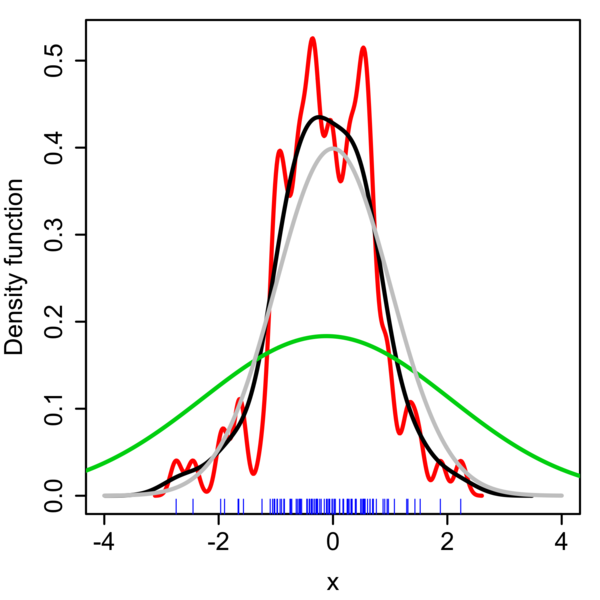
\includegraphics[width=0.5\textwidth]{bandwidth_selectors.png}
    \caption{The blue marks at the bottom of the plot shows a random sample from the Gaussian distribution. The grey curve shows the true density. The red curve visualises an undersmoothed estimation. The green curve visualises an oversmoothed estimation. The black curve is estimated using a near optimal bandwidth~\cite{wiki:kernel_density_estimation}.}
    \label{fig:bandwidth_selectors}
\end{figure}

\subsubsection{Finding a Good Bandwidth}

Finding the perfect bandwidth can be difficult. Which metrics define how good a given bandwidth is, depends on the domain of the data.

A simple approach is to eye-ball the results of using a variety of bandwidths. The result that gives the best looking bandwidth would then be chosen. This approach can give perfectly acceptable bandwidths, but the analyser has to have domain knowledge of the data. The results of this method are not reproducible, as different analysts will not deterministically choose their optimal bandwidths. Furthermore, it is also a tedious process.

Another approach is to choose a bandwidth based on a metric of minimal errors. The idea is that an optimal solution will have the least errors. One method of doing this is to find the bandwidth with the lowest mean integrated squared error (MISE), as shown in \cref{eq:mise}.

\begin{equation}\label{eq:mise}
     E \int(\hat f_{h}(x) - f(x) )^2\mathrm{d}x
\end{equation}

In this method we take the integral of the squared difference between the estimate function $\hat f$ given bandwidth $h$ and the true density function $f$. We then multiply this with the expected mean value $E$ for the true density data. The intuition is that the bandwidth which will give the lowest area of error should be chosen. The hardest part of this method is to identify $f$.

As noted in the introduction to this section, we will do a very simple bandwidth selection experiment. We therefore use a simpler metric of error called the sum of squared error (SSE). The SSE is defined in \cref{eq:sse}.

\begin{equation}\label{eq:sse}
    \sum (\hat f_{h}(x) - f(x) )^2
\end{equation}

Here $\hat f_{h}(x)$ is the kernel density estimator $\hat f$ with bandwidth $h$ for a point $x$  and $f(x)$ is the actual density at point $x$. The idea of is to find the bandwidth that minimises the SSE.

The SSE formula defined in \cref{eq:sse} needs true density test data to be used as a benchmark for the performance of the bandwidth. In the perfect world, this test data should have the same structure as a real world crowd. We consider the problem of finding test data that matches a real world crowd as difficult, maybe even suitable for a project on its own. Instead, we will generate a simple pattern, that will illustrate how different bandwidths affect the kernel density estimation results.

We generate test data that takes the pattern of a chess board. This means that people has been placed such that the square alternates between two densities. The true densities are illustrated in \cref{fig:chessBoard-low1-high3-band5} where the blue squares have a density of 1 person per square metre and the turquoise squares have a density of 3 persons per square metre.

\definecolor{lowDensity}{HTML}{0967FD}
\definecolor{highDensity}{HTML}{00FFCF}

\begin{figure}[htbp]
\centering
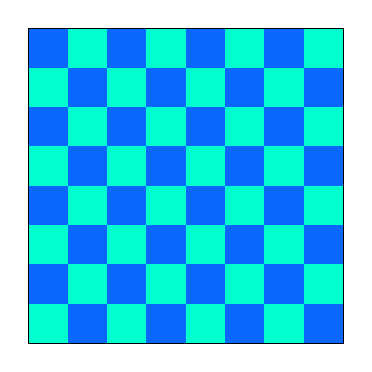
\begin{tikzpicture}[x=1cm,scale=0.5]
    \foreach \x in {0,...,7} \foreach \y in {0,...,7}
    {
        \pgfmathparse{mod(\x+\y,2) ? "lowDensity" : "highDensity"}
        \edef\colour{\pgfmathresult}
        \path[fill=\colour] (\x,\y) rectangle ++ (1,1);
    }
    \draw (0,0)--(0,8)--(8,8)--(8,0)--cycle;
\end{tikzpicture}
    \caption{Chess board pattern with blue squares having a density of 1 person per square meter and turquoise squares having a density of 3 person per square meter.}
    \label{fig:chessBoard-low1-high3-band5}
\end{figure}

The next section will give concrete data that shows how different bandwidths affect the density estimation.

\subsubsection{Effect of Bandwidth}

Using the chess board pattern introduced in the previous section, we will now get a better intuition of the choice of bandwidth. 

\begin{figure}[htbp]
\centering

\begin{subfigure}[c]{.32\linewidth}
    \centering
    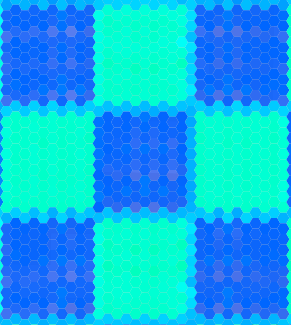
\includegraphics[width=\textwidth]{chessBoard-low1-high3-band1-density-subsquares.png}
    \caption{Bandwidth 1 metre}
    \label{fig:chessBoard-low1-high3-band1-cropped}
\end{subfigure}
%
\begin{subfigure}[c]{.32\linewidth}
    \centering
    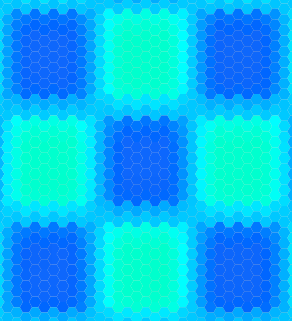
\includegraphics[width=\textwidth]{chessBoard-low1-high3-band5-density-subsquares.png}
    \caption{Bandwidth 5 metre}
    \label{fig:chessBoard-low1-high3-band5-cropped}
\end{subfigure}
%
\begin{subfigure}[c]{.32\linewidth}
    \centering
    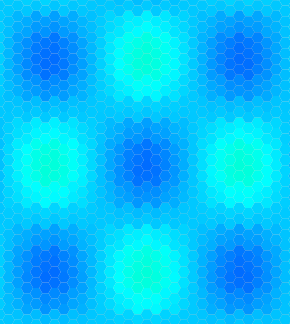
\includegraphics[width=\textwidth]{chessBoard-low1-high3-band10-density-subsquares.png}
    \caption{Bandwidth 10 metre}
    \label{fig:chessBoard-low1-high3-band10-cropped}
\end{subfigure}
%
\caption{Cropped chess board pattern with blue squares having a density of 1 and turquoise squares having a density of 3. The bandwidth varies on the different subfigures.}
\label{fig:chessBoard-different-bandwidths}
\end{figure}

Let's look at how three different bandwidths change the kernel density estimation of the same data set. \Cref{fig:chessBoard-different-bandwidths} depicts three chess board patterns with varying bandwidths. \Cref{fig:chessBoard-low1-high3-band1-cropped} is very close to the structure of the chess board pattern, but there is some unwanted noise in the blue squares. We would say that the estimation is a little undersmoothed. \Cref{fig:chessBoard-low1-high3-band5-cropped} has a more blurry transition between each adjacent square, which means that the estimation is not really finding the hard transition of the underlying true data. There is however no noise inside each square. We would say that the estimation is a little oversmoothed. In \cref{fig:chessBoard-low1-high3-band10-cropped} we see a clear example of an oversmoothing bandwidth. Each square transition is still somewhat visible, but it is nowhere near the underlying true data.

Every bandwidth in \cref{fig:chessBoard-different-bandwidths} had some problems; Either the bandwidth was too low or too high. We will now try to determine a better bandwidth using the aforementioned SSE method. We iterate through a bandwidth interval from 1 metre to 5 metres with a step of 0.1 metre, because we know that the optimal bandwidth is around that interval. The result of the calculation is that the best bandwidth is 1.4 metre with an SSE of $5745.06$. \Cref{fig:chessBoard-low1-high3-band1.4-cropped} shows a crop of the chess board data with a bandwidth of 1.4 metre. We can see that this bandwidth indeed seems to be optimal; There is no noise inside the blue squares, and the square transitions are still following the underlying structure of the true density data.

\begin{figure}[htbp]
\centering
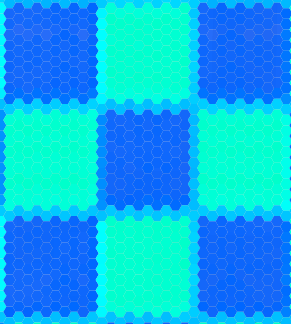
\includegraphics[width=0.32\textwidth]{chessBoard-low1-high3-band1-4-density-subsquares.png}
\caption{Cropped chess board pattern with blue squares having a density of 1 and turquoise squares having a density of 3. The bandwidth of 1.4 metres is calculated using a SSE method.}
\label{fig:chessBoard-low1-high3-band1.4-cropped}
\end{figure}

\subsubsection{Summary}

The above sample data is useful for giving an intuition of the effect of different bandwidths, but in order for the bandwidth selection to be useful in practice, one would have to do the bandwidth selection on data that represents the crowd to be analysed.